\documentclass[]{article}

\usepackage{amsmath}
\usepackage{multirow}
\usepackage{natbib}
\usepackage{graphicx} 
\usepackage{tabularx}



\begin{document}

\title{The Conditional Predictive Power of Sectoral Volatility Dispersion for VIX Innovations}

\author{Denario}
\date{Anthropic, Gemini \& OpenAI servers. Planet Earth.}

\maketitle
\begin{abstract}
This study investigates whether the cross-sectional dispersion of realized volatility across market sectors can serve as a leading indicator for shifts in the CBOE Volatility Index (VIX), a critical challenge in risk management. We construct a daily Sectoral Volatility Dispersion (SVD) metric from ten US sector ETFs spanning 2015 to 2026 and employ a Hidden Markov Model to endogenously classify VIX regimes. Econometric analysis reveals that SVD, in isolation, is not a statistically significant predictor of future VIX innovations or transitions into high-volatility states. However, we uncover a crucial conditional relationship: the predictive power of SVD emerges only when it interacts with market structure. Specifically, elevated SVD is significantly associated with higher 21-day ahead VIX innovations only when accompanied by a breakdown in average cross-sector correlation. These findings indicate that cross-sectional dispersion should not be interpreted as a standalone timing signal, but rather as a component of a more nuanced market fragility indicator, where the combination of idiosyncratic volatility and sector decoupling signals heightened vulnerability to systemic risk.
\end{abstract}








\section{Introduction}
\label{sec:intro}
Anticipating shifts in systemic risk is a foundational challenge in financial economics, with the CBOE Volatility Index (VIX) serving as the principal barometer of expected market-wide turmoil. While many forecasting models rely on aggregate market data, valuable precursory information may lie latent within the market's internal structure. The dynamics of how different economic sectors behave relative to one another can offer insight into the underlying stability of the financial system, raising a critical question: can the divergence in the risk profiles of individual sectors provide a leading signal for future changes in aggregate market volatility?

The central problem this paper addresses is the ambiguity inherent in measures of cross-sectional volatility dispersion. An increase in the dispersion of realized volatility across sectors—where some parts of the market become significantly more turbulent than others—can be interpreted in two distinct ways. It could represent benign, idiosyncratic noise confined to specific industries, or it could be a symptom of rising market fragility, where underlying economic stressors affect sectors heterogeneously before coalescing into a systemic event. Distinguishing between these two interpretations is crucial for developing reliable risk-monitoring tools that can filter meaningful signals from market noise.

To resolve this ambiguity, we propose and test a conditional framework. We first construct a daily metric, termed Sectoral Volatility Dispersion (SVD), calculated as the cross-sectional standard deviation of 21-day realized volatilities across ten major US sector ETFs. Our central hypothesis is that the predictive power of SVD for future VIX innovations is not absolute but is contingent on the market's broader correlational structure. Specifically, we posit that elevated SVD only becomes a potent indicator of impending systemic risk when it is accompanied by a breakdown in the market's internal cohesion, measured by the average cross-sector correlation. This approach frames market fragility not just as a function of rising idiosyncratic risk, but as the simultaneous occurrence of such risk and the decoupling of its constituent parts.

Our empirical investigation, which employs a Hidden Markov Model to endogenously classify VIX regimes, provides strong support for this conditional relationship. We find that SVD, when considered in isolation, is not a statistically significant predictor of future VIX innovations or the probability of transitioning into a high-volatility state. However, its predictive power emerges robustly through its interaction with market structure. Elevated SVD is significantly associated with higher 21-day ahead VIX innovations, but only when average cross-sector correlation is low. This study contributes by clarifying that cross-sectional volatility dispersion should not be interpreted as a standalone timing signal. Instead, it is a critical component of a more sophisticated indicator of market fragility, where the combination of high idiosyncratic volatility and sector decoupling signals a heightened vulnerability to future market-wide stress.

\section{Methods}
\label{sec:methods}
\subsection{Data and Feature Construction}
The primary dataset consists of daily closing prices for nine major US sector ETFs (XLK, XLF, XLV, XLE, XLI, XLY, XLP, XLU, XLB) and the CBOE Volatility Index (VIX) from January 2015 to April 2026. The S\&P 500 index (\textasciicircum GSPC) was also included as a market-wide control variable. All data was processed to ensure a balanced panel by removing days with missing observations for any of the assets.

The core metric, Sectoral Volatility Dispersion (SVD), was constructed through a multi-step process. First, daily logarithmic returns were calculated for each of the nine sector ETFs. Second, for each ETF, we computed a 21-day rolling realized volatility, defined as the standard deviation of its log-returns over the preceding 21 trading days. This daily volatility figure was then annualized:
\begin{equation}
    \sigma_{i,t}^{(21)} = \sqrt{252} \times \text{StDev}(r_{i, t-20:t})
\end{equation}
where $\sigma_{i,t}^{(21)}$ is the annualized 21-day realized volatility for sector $i$ at day $t$, and $r_{i, t-20:t}$ is the series of daily log-returns for that sector over the 21-day window.

The SVD for each day $t$ was then calculated as the cross-sectional standard deviation of these nine concurrent realized volatility estimates:
\begin{equation}
    \text{SVD}_t = \sqrt{\frac{1}{N-1} \sum_{i=1}^{N} (\sigma_{i,t}^{(21)} - \bar{\sigma}_{t}^{(21)})^2}
\end{equation}
where $N=9$ is the number of sectors and $\bar{\sigma}_{t}^{(21)}$ is the cross-sectional average of the sector volatilities at time $t$. To ensure stationarity and facilitate interpretation in our regression models, this raw SVD series was transformed into a normalized Z-score using a rolling 252-day (one trading year) lookback window for the mean and standard deviation. Stationarity of the resulting time series was confirmed using the Augmented Dickey-Fuller (ADF) test.

To capture the market's correlational structure, we also computed a daily measure of average cross-sector correlation. This was calculated as the mean of all unique pairwise correlations across the nine sector ETFs, based on their daily returns over a rolling 21-day window.

\subsection{VIX Regime Identification}
To endogenously classify market volatility states, we employed a three-state Gaussian Hidden Markov Model (HMM). This probabilistic approach avoids the use of arbitrary, fixed thresholds for the VIX and instead allows the data to define distinct regimes based on the distributional properties of VIX changes. The model was fitted to the daily log-returns of the VIX index, $\Delta \ln(\text{VIX}_t) = \ln(\text{VIX}_t / \text{VIX}_{t-1})$, to ensure the input series was stationary. The three latent states identified by the HMM were subsequently labeled as ``Low'', ``Moderate'', and ``High'' volatility regimes by examining the average raw VIX level corresponding to the days classified within each state.

\subsection{Econometric Analysis}
Our empirical investigation involved two primary modeling frameworks to assess the predictive power of SVD.

First, to test the conditional relationship between SVD and future VIX movements, we estimated an Ordinary Least Squares (OLS) regression model. The model predicts the $k$-day ahead log-return of the VIX using the normalized SVD, an interaction term between SVD and the average sector correlation, and several control variables. The full specification is:
\begin{equation}
    \Delta \ln(\text{VIX})_{t+k} = \alpha + \beta_1 \text{SVD}_t + \beta_2 (\text{SVD}_t \times \text{AvgCorr}_t) + \beta_3 \Delta \ln(\text{VIX})_t + \beta_4 r_{\text{MKT},t} + \epsilon_t
\end{equation}
where $\Delta \ln(\text{VIX})_{t+k}$ is the log-return of the VIX over the next $k$ days, $\text{SVD}_t$ is the normalized SVD at time $t$, $\text{AvgCorr}_t$ is the 21-day average sector correlation, $\Delta \ln(\text{VIX})_t$ is the concurrent VIX log-return, and $r_{\text{MKT},t}$ is the concurrent S\&P 500 log-return. We estimated this model for horizons of $k=5$ and $k=21$ days. To ensure robust statistical inference in the presence of heteroskedasticity and autocorrelation inherent in overlapping time-series data, all reported standard errors were corrected using the Newey-West estimator.

Second, to evaluate SVD as a discrete warning signal for regime shifts, we used a logistic regression model. The model was designed to predict the probability of the market transitioning into the ``High'' volatility regime on day $t$, conditional on not being in that state on day $t-1$. The primary predictor was the lagged normalized SVD ($SVD_{t-1}$). Model performance was evaluated using two metrics: the Area Under the Receiver Operating Characteristic curve (AUROC), which measures overall discriminatory power, and the Precision-Recall Area Under the Curve (PR AUC), which is more informative for evaluating classifiers on highly imbalanced datasets where the event of interest (a transition to high volatility) is rare.

Finally, to confirm that our findings were not driven by the behavior of any single sector, we performed a Leave-One-Out Cross-Validation (LOOCV) on the logistic regression model. The SVD metric was recalculated nine times, each time excluding one sector ETF, and the AUROC was computed for each iteration to assess the stability of the model's predictive performance.

\section{Results}
\label{sec:results}
This section presents the empirical findings from our investigation into Sectoral Volatility Dispersion (SVD) as a leading indicator for innovations in the CBOE Volatility Index (VIX). The analysis spans from January 2015 to April 2026. We first characterize the VIX regimes and the dynamics of our dispersion metric, then present the results from our econometric models assessing the conditional predictive power of SVD.

\subsection{VIX regimes and dispersion dynamics}
The foundational metric of this study, Sectoral Volatility Dispersion (SVD), was constructed as the cross-sectional standard deviation of 21-day realized volatilities across nine major sector ETFs. To facilitate time-series modeling, this raw measure was transformed into a rolling 252-day Z-score. An Augmented Dickey-Fuller (ADF) test confirmed that the normalized SVD series is stationary (ADF statistic = -4.97, $p < 0.001$), making it a suitable candidate for our predictive models.

To define market states, we applied a three-state Gaussian Hidden Markov Model (HMM) to the daily log-returns of the VIX. This data-driven approach avoids arbitrary thresholds and identifies regimes based on the distributional properties of VIX changes. By examining the average VIX level on days assigned to each latent state, we labeled the regimes as:
\begin{itemize}
    \item \textbf{Low Volatility Regime:} Mean VIX of 17.54
    \item \textbf{Moderate Volatility Regime:} Mean VIX of 19.29
    \item \textbf{High Volatility Regime:} Mean VIX of 21.90
\end{itemize}
The elevated baseline of the "Low" regime reflects the structural characteristics of the post-2015 sample period, which included several episodes of heightened market tension.

Figure \ref{fig:vix_svd_corr} visualizes the temporal evolution of the VIX and its HMM-defined regimes alongside the normalized SVD and the average 21-day cross-sector correlation. Visual inspection suggests that spikes in SVD often coincide with or slightly precede transitions into the High volatility regime. However, this relationship appears inconsistent and potentially modulated by the concurrent state of cross-sector correlation, motivating a more rigorous econometric analysis.

\begin{figure*}[t]
    \centering
    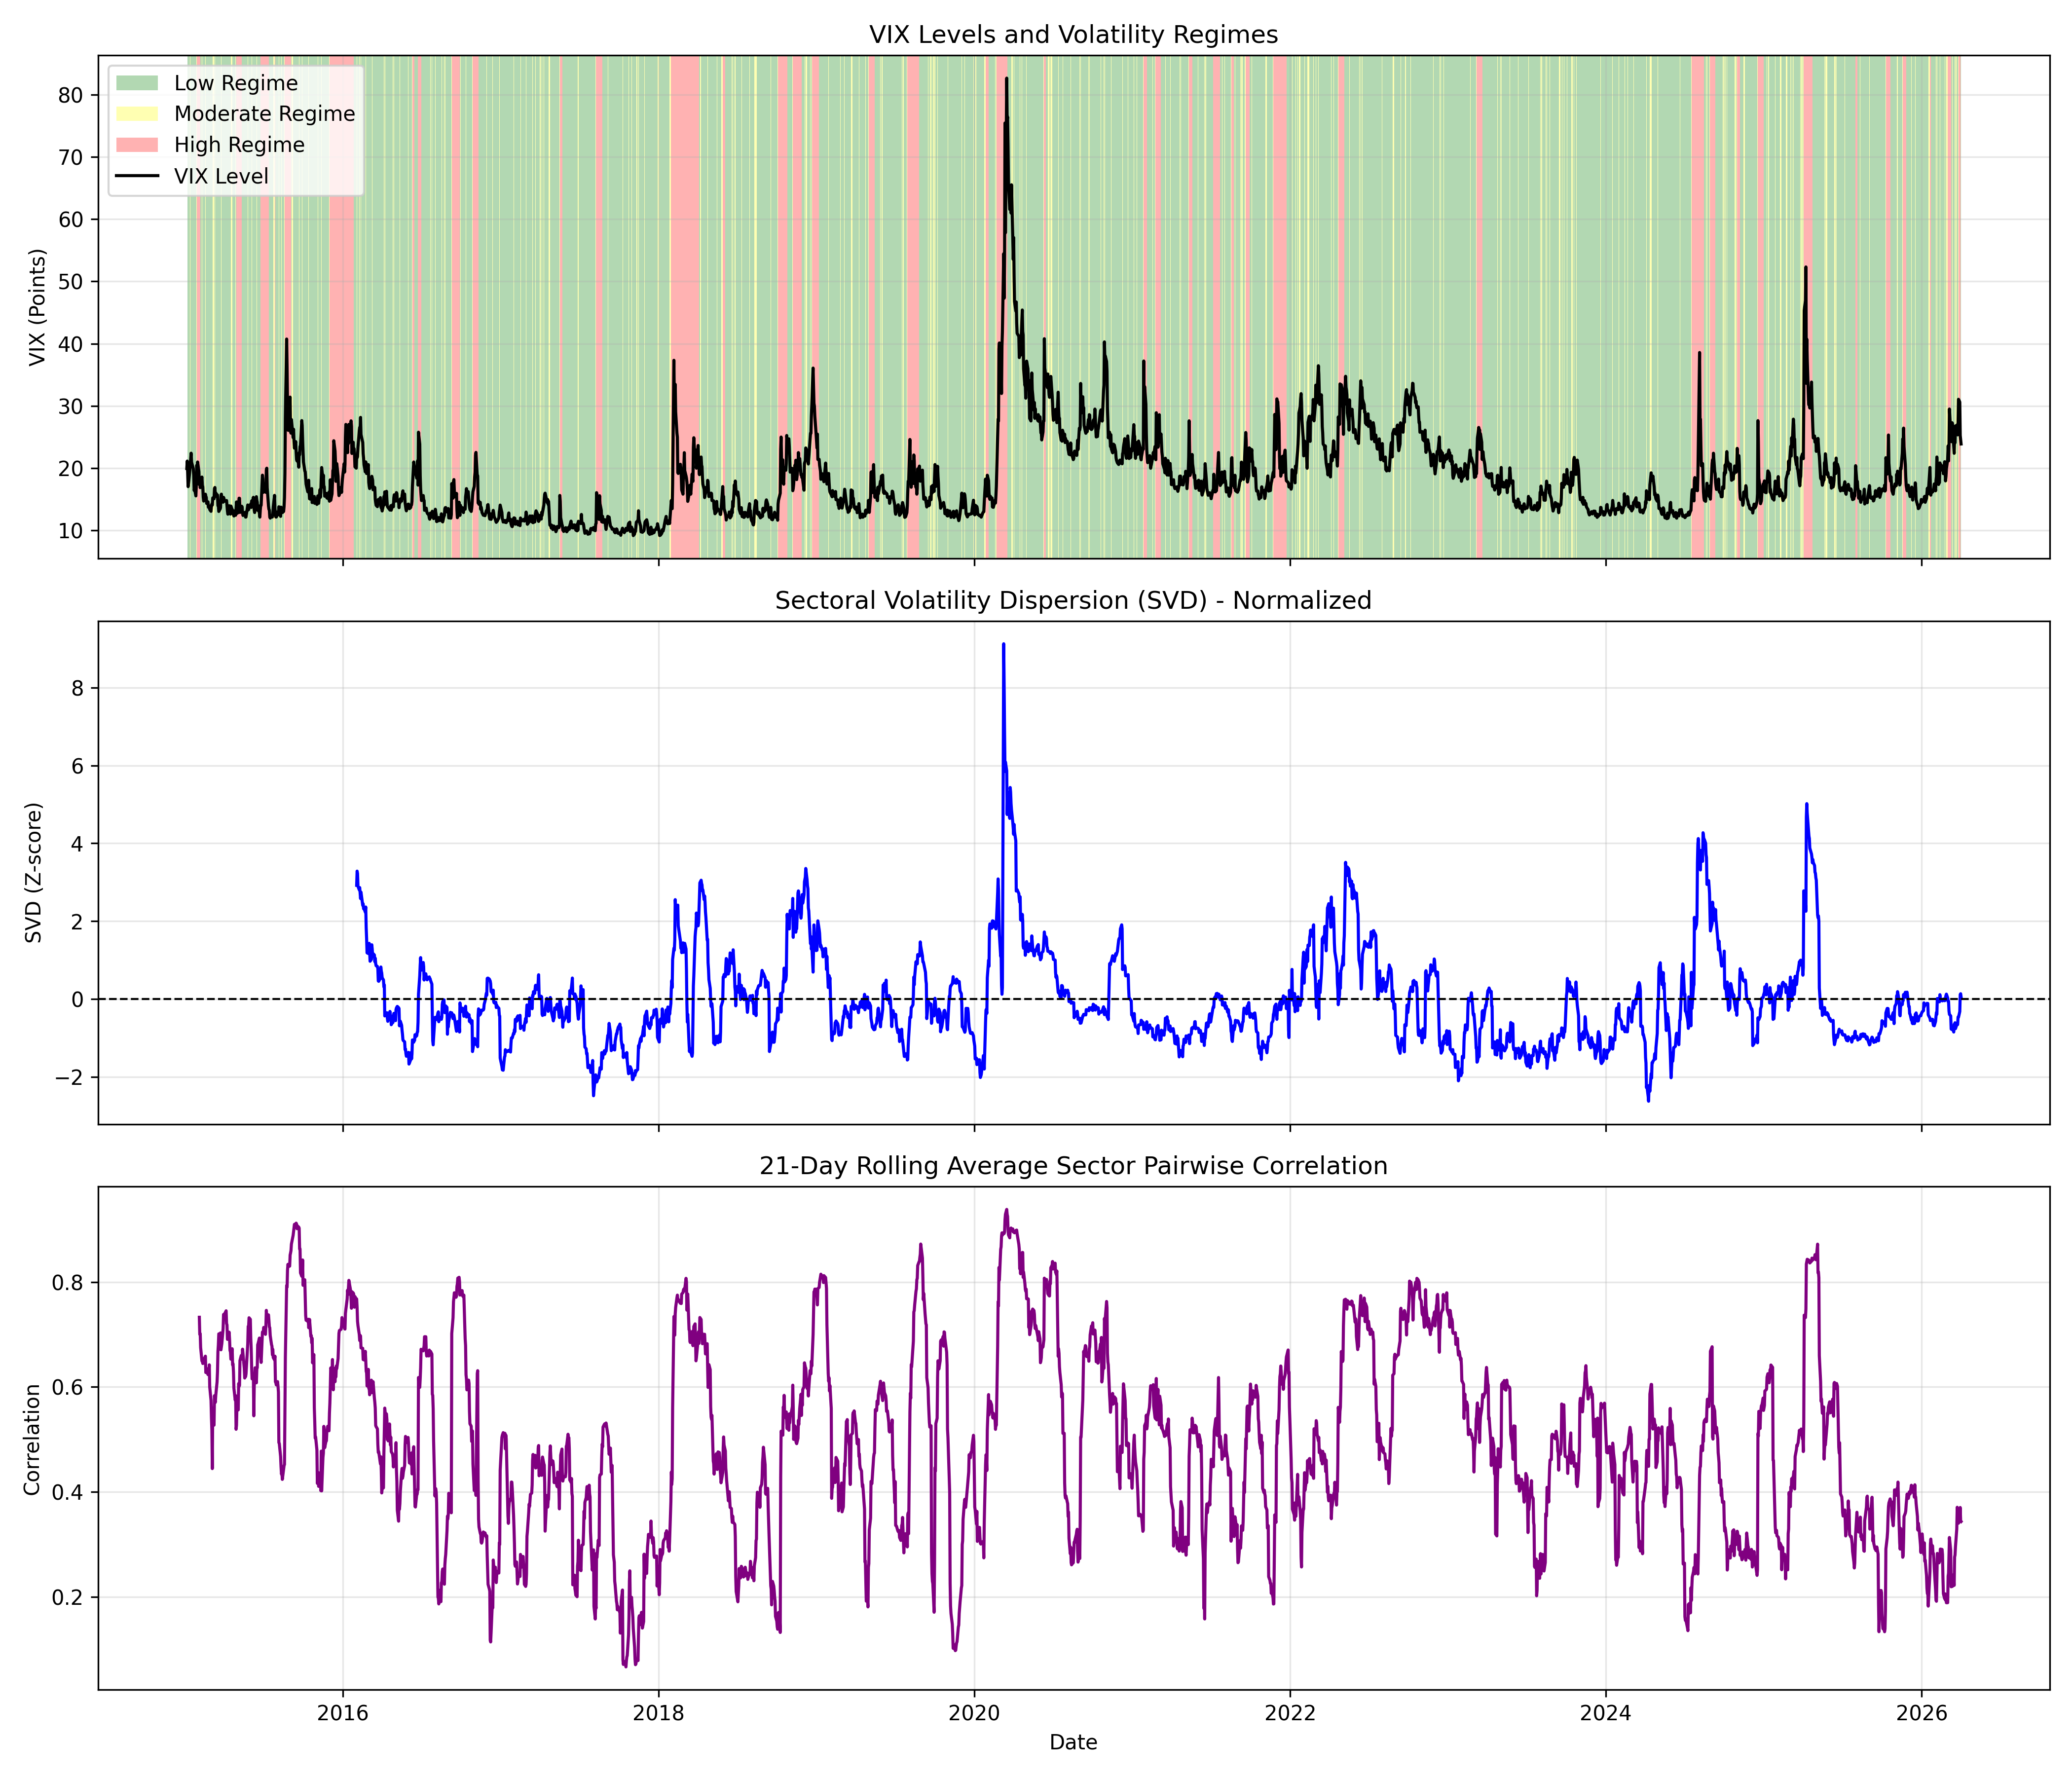
\includegraphics[width=\textwidth]{../input_files/plots/step_5_vix_svd_correlation_multipanel_1_20260406_094306.png}
    \caption{Temporal evolution of key market metrics from January 2015 to April 2026. The top panel displays the CBOE Volatility Index (VIX) with background shading indicating the Low, Moderate, and High volatility regimes identified by a Hidden Markov Model. The middle panel shows the normalized Sectoral Volatility Dispersion (SVD), a 252-day rolling Z-score of the cross-sectional standard deviation of sector volatilities. The bottom panel plots the 21-day rolling average of pairwise sector correlations. The visualization suggests that spikes in SVD frequently coincide with or precede transitions into the High volatility regime, a relationship that appears to be modulated by the concurrent state of cross-sector correlation.}
    \label{fig:vix_svd_corr}
\end{figure*}

\subsection{The conditional predictive power of SVD}
To formally test our central hypothesis, we estimated an Ordinary Least Squares (OLS) regression to predict future VIX log-returns at 5-day and 21-day horizons. The model included normalized SVD, an interaction term between SVD and average sector correlation, and standard control variables. Standard errors were corrected using the Newey-West estimator to account for autocorrelation and heteroskedasticity.

The results are summarized in Table \ref{tab:ols_results}. At the short-term 5-day horizon, the model has weak explanatory power ($R^2 = 0.016$), and neither SVD nor its interaction with correlation is statistically significant. The only significant predictor is the concurrent market return, reflecting the well-documented contemporaneous leverage effect.

\begin{table*}[t]
\centering
\caption{OLS Regression of Future VIX Log-Returns}
\label{tab:ols_results}
\resizebox{\textwidth}{!}{
\begin{tabular}{l c c c c}
\hline\hline
 & \multicolumn{2}{c}{5-Day Ahead $\Delta \ln(\text{VIX})$} & \multicolumn{2}{c}{21-Day Ahead $\Delta \ln(\text{VIX})$} \\
\cline{2-3} \cline{4-5}
Variable & Coefficient & p-value & Coefficient & p-value \\
\hline
Intercept & 0.0031 & (0.849) & -0.0058 & (0.831) \\
SVD$_t$ & -0.0014 & (0.944) & 0.0473 & (0.198) \\
SVD$_t \times$ AvgCorr$_t$ & -0.0128 & (0.690) & \textbf{-0.1267} & \textbf{(0.013)} \\
$\Delta \ln(\text{VIX})_t$ & -0.0495 & (0.118) & -0.0911 & (0.052) \\
$r_{\text{MKT},t}$ & \textbf{1.0832} & \textbf{(0.012)} & 0.8954 & (0.145) \\
\hline
Observations & \multicolumn{2}{c}{2,828} & \multicolumn{2}{c}{2,828} \\
$R^2$ & \multicolumn{2}{c}{0.016} & \multicolumn{2}{c}{0.047} \\
\hline
\multicolumn{5}{l}{\footnotesize Note: Standard errors are Newey-West corrected. Bold values indicate statistical significance at the 5\% level.}
\end{tabular}
}
\end{table*}

In contrast, at the 21-day horizon, a crucial dynamic emerges. While the SVD term in isolation remains statistically insignificant ($p = 0.198$), the interaction term between SVD and average sector correlation is negative and highly significant ($\beta = -0.1267$, $p = 0.013$). This is the central finding of our study. The negative coefficient implies that the effect of SVD on future VIX innovations is conditional on the market's correlational structure. Specifically, an increase in SVD is associated with significantly higher 21-day ahead VIX innovations only when average sector correlation is low. When correlation is high, the effect of SVD is dampened or reversed. This result supports our hypothesis that SVD is not a standalone signal but becomes a potent indicator of market fragility when it coincides with a breakdown in the market's internal cohesion.

\subsection{SVD as a regime transition warning signal}
We next evaluated SVD's utility as a discrete warning signal for imminent volatility spikes using a logistic regression model. The model was designed to predict the probability of transitioning into the "High" volatility regime on day $t$, conditional on not being in that state on day $t-1$. The primary predictor was the lagged normalized SVD.

The model failed to find a significant relationship, with the coefficient for lagged SVD being statistically insignificant ($p = 0.558$). The model's overall discriminatory power, shown in Figure \ref{fig:logreg_performance}, is poor. The Area Under the Receiver Operating Characteristic curve (AUROC) is 0.526, only marginally better than a random guess (0.500). More revealing is the Precision-Recall Area Under the Curve (PR AUC), which is a more informative metric for imbalanced datasets where the event of interest (a transition to high volatility) is rare. The PR AUC of 0.02 is exceptionally low, indicating that when the model does predict a transition, it has very low precision. This result reinforces the finding from our linear models: SVD, when considered in isolation, is not an effective tool for timing discrete shifts into high-volatility states.

\begin{figure*}[t]
    \centering
    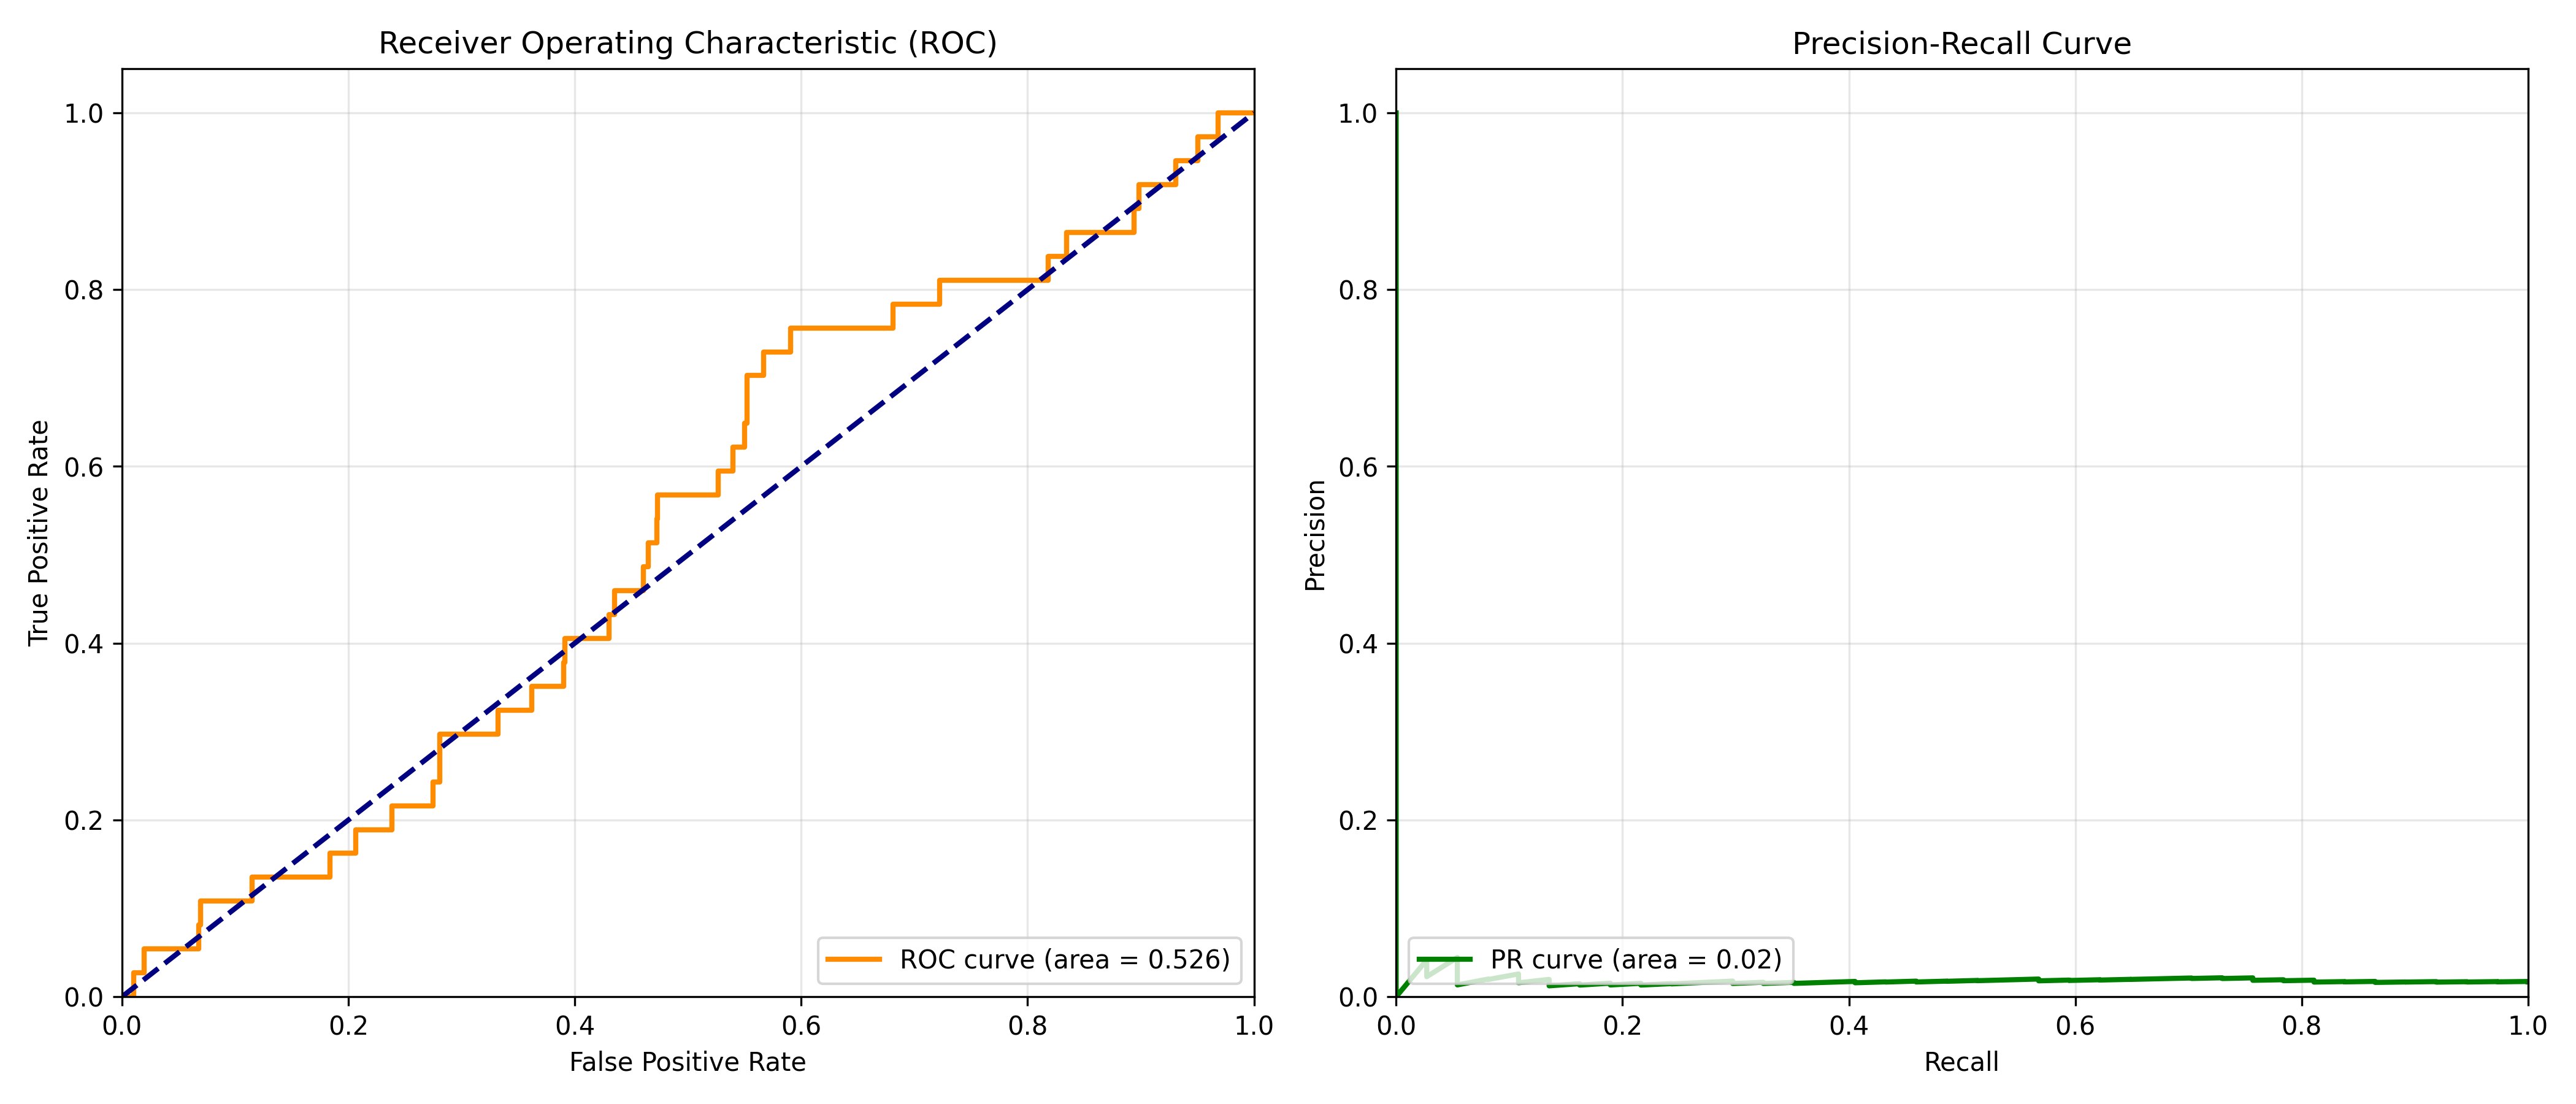
\includegraphics[width=\textwidth]{../input_files/plots/step_5_model_performance_curves_2_20260406_094306.png}
    \caption{Performance of the logistic regression model designed to predict transitions into the High VIX regime using lagged normalized Sectoral Volatility Dispersion (SVD). The left panel displays the Receiver Operating Characteristic (ROC) curve, yielding an Area Under the Curve (AUROC) of 0.526, which indicates predictive power only marginally better than a random classifier. The right panel presents the Precision-Recall (PR) curve, whose area of 0.02 highlights the model's poor performance. This extremely low PR AUC, driven by the severe class imbalance of rare regime transitions, demonstrates that SVD in isolation is an insufficient predictor for the timing of VIX regime shifts.}
    \label{fig:logreg_performance}
\end{figure*}

\subsection{Robustness to sectoral composition}
To ensure our findings were not driven by the idiosyncratic behavior of a single dominant sector (e.g., Technology or Energy), we performed a Leave-One-Out Cross-Validation (LOOCV) on the logistic regression model. The SVD metric was recalculated nine times, each time excluding one sector, and the model's AUROC was re-evaluated.

The results, presented in Figure \ref{fig:loocv_robustness}, demonstrate the stability of our conclusions. The AUROC scores are tightly clustered around the baseline model's performance, with a mean of 0.527 and a standard deviation of just 0.009. This narrow distribution confirms that the informational content of SVD—and its limitations as an unconditional predictor—is a robust, market-wide phenomenon. The signal is genuinely cross-sectional and not an artifact of any single sector's variance.

\begin{figure}[h!]
    \centering
    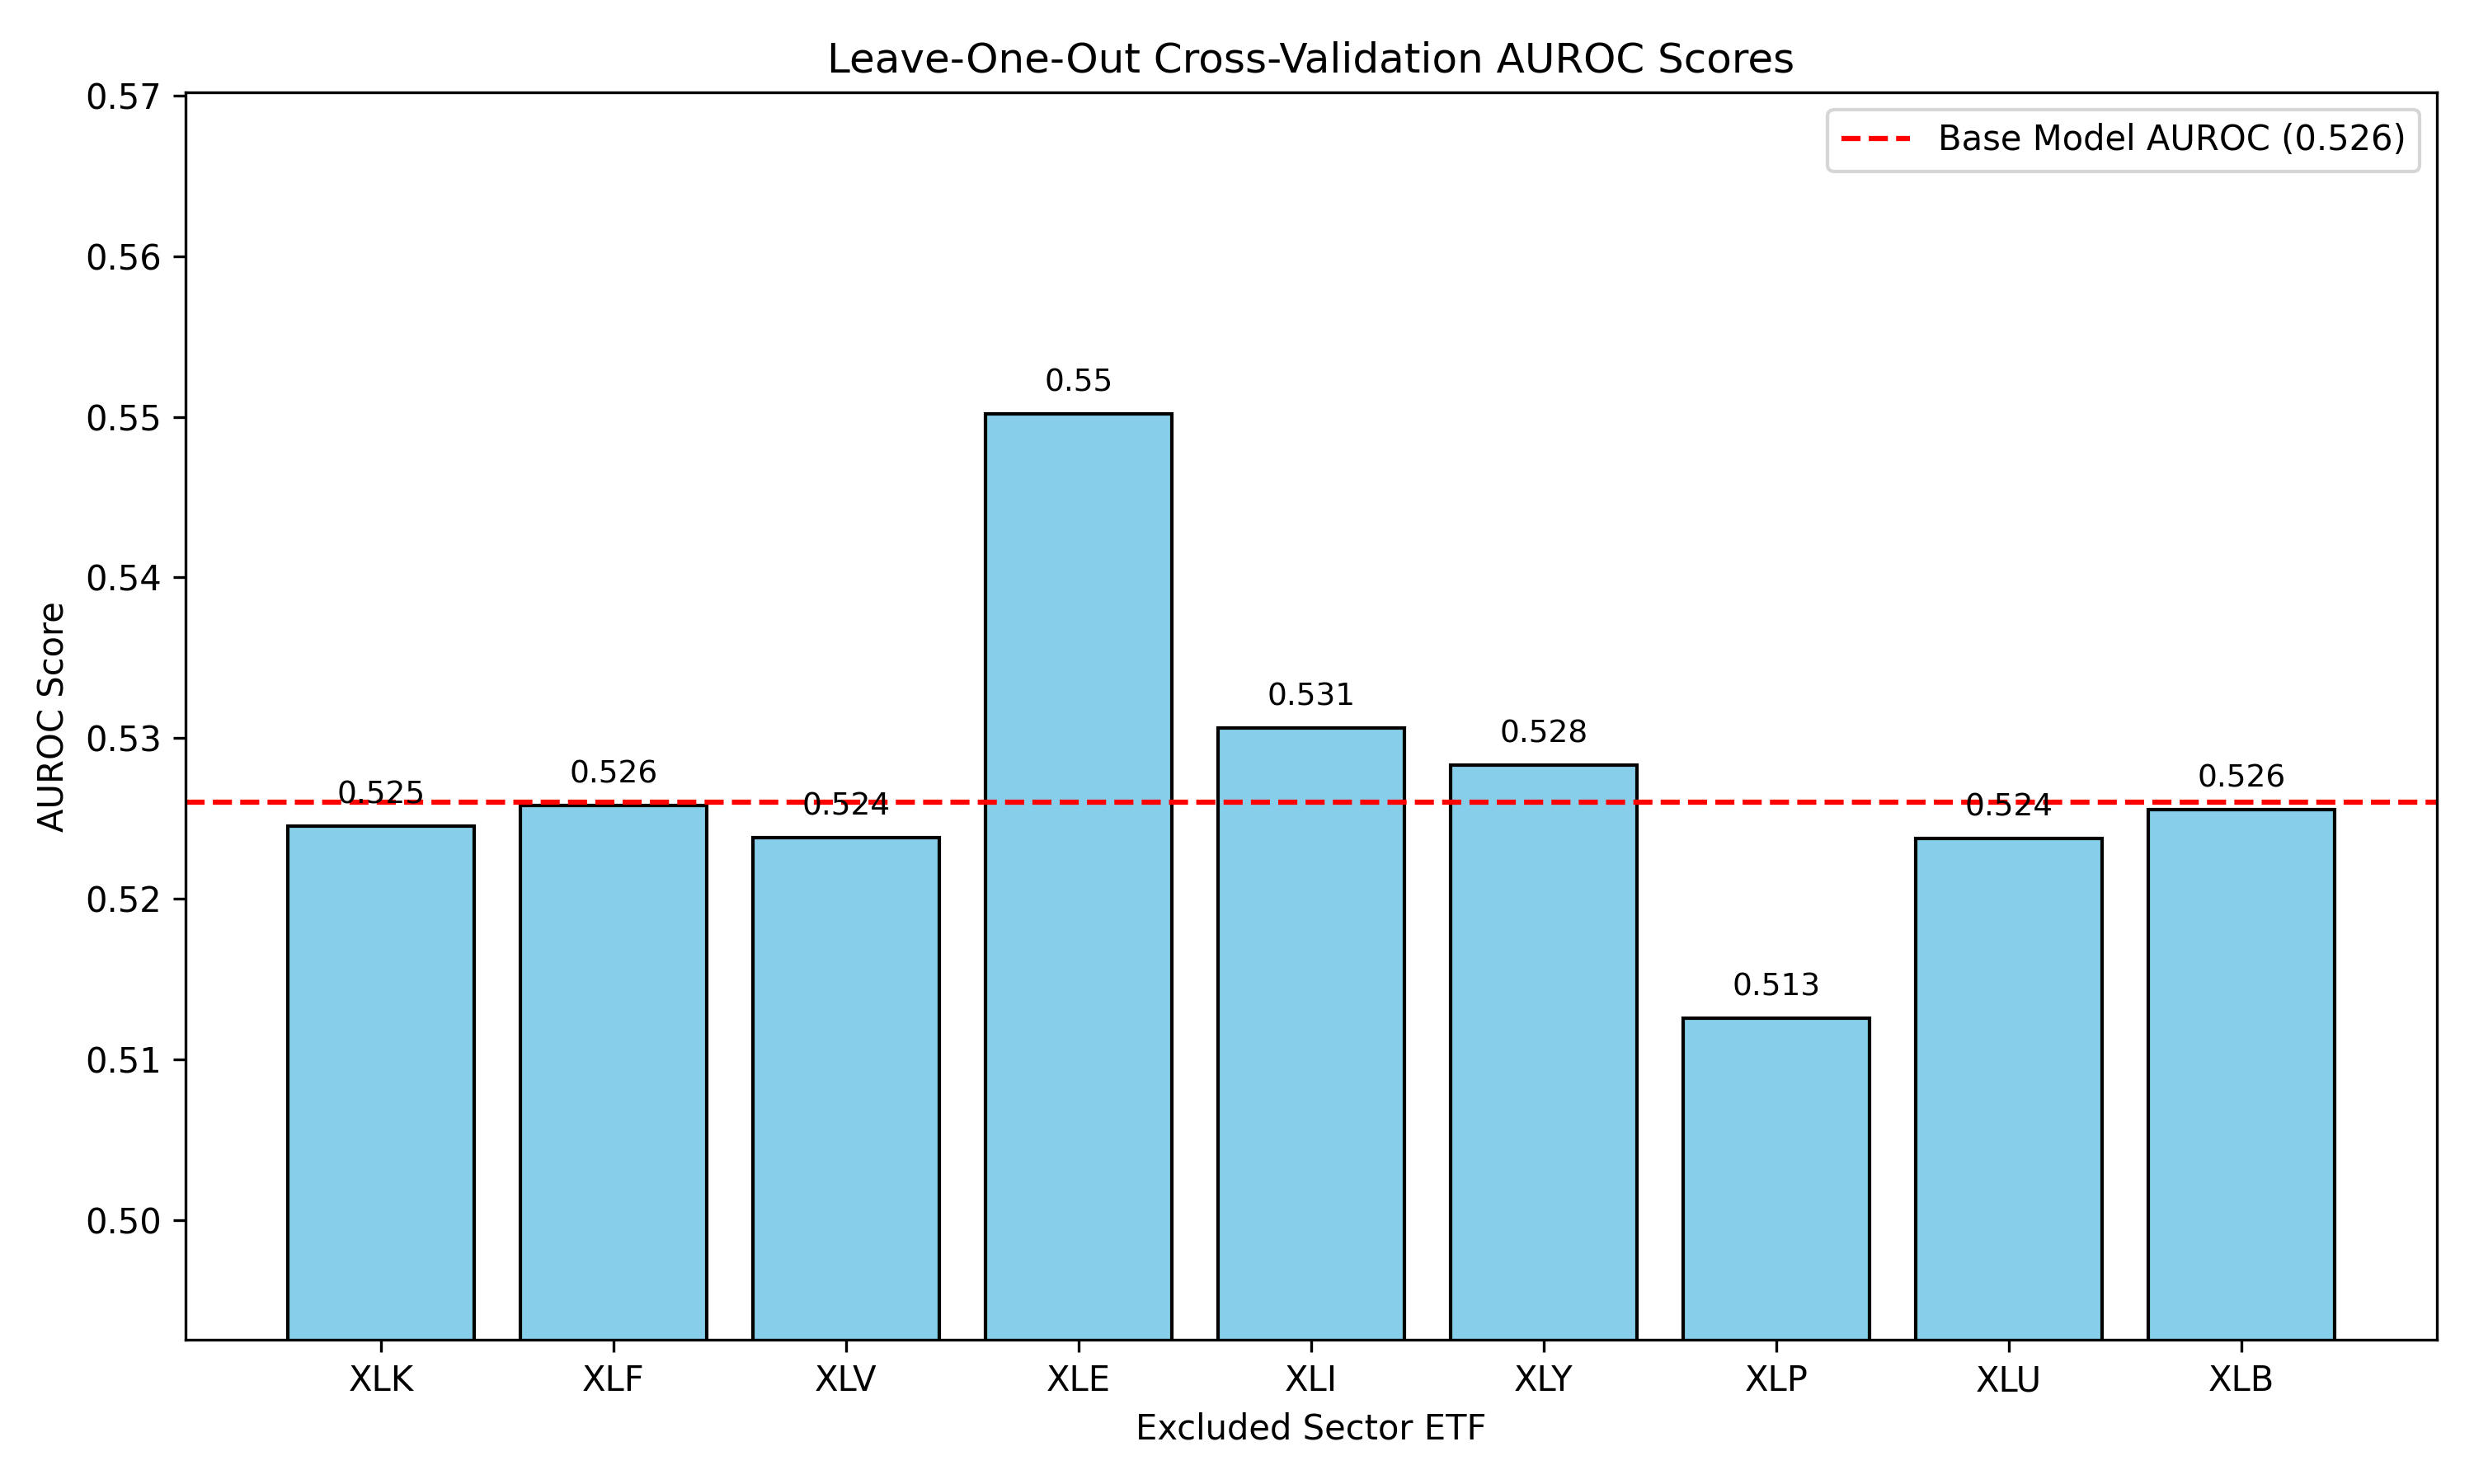
\includegraphics[width=0.5\textwidth]{../input_files/plots/step_5_loocv_auroc_barchart_3_20260406_094306.png}
    \caption{Robustness of the Sectoral Volatility Dispersion (SVD) metric assessed via a Leave-One-Out Cross-Validation (LOOCV) procedure. The bar chart displays the Area Under the Receiver Operating Characteristic (AUROC) score for the logistic regression model predicting VIX regime transitions, where the SVD metric is iteratively recalculated excluding one of the nine sector ETFs. The tight clustering of the AUROC scores around the baseline model's performance (0.526, red dashed line) demonstrates that the informational content and predictive limitations of SVD are a robust, market-wide phenomenon and not an artifact driven by any single sector's volatility.}
    \label{fig:loocv_robustness}
\end{figure}

\section{Conclusions}
\label{sec:conclusions}
This study investigated whether the cross-sectional dispersion of realized volatility across market sectors can serve as a leading indicator for shifts in the CBOE Volatility Index (VIX). The central problem addressed was the inherent ambiguity in such dispersion metrics: whether they represent benign, idiosyncratic sector-specific noise or a symptom of rising market fragility that precedes systemic turmoil. We hypothesized that the predictive power of dispersion is not absolute but is conditional on the market's broader correlational structure.

To test this, we constructed a daily Sectoral Volatility Dispersion (SVD) metric using data from nine major US sector ETFs from 2015 to 2026. We employed a three-state Hidden Markov Model to endogenously classify VIX regimes and used Ordinary Least Squares (OLS) and logistic regression models to assess the predictive power of SVD. The OLS model included a key interaction term between SVD and the average cross-sector correlation to test our conditional hypothesis.

Our empirical results deliver a clear and nuanced conclusion. We found that SVD, when considered in isolation, is not a statistically significant predictor of future VIX innovations or the probability of transitioning into a high-volatility state. A logistic regression model designed to time these regime shifts performed poorly, with an AUROC of just 0.526, indicating its ineffectiveness as a standalone warning signal. However, our central finding, derived from the OLS regression, reveals a significant conditional relationship. At a 21-day forecast horizon, the interaction between SVD and average sector correlation was found to be a statistically significant predictor of VIX innovations.

From these results, we have learned that the informational content of sectoral volatility dispersion is context-dependent. An increase in SVD is associated with significantly higher future market volatility only when it is accompanied by a breakdown in the market's internal cohesion, as measured by low average cross-sector correlation. When sectors remain highly correlated, high dispersion does not signal impending systemic risk. This study clarifies that cross-sectional dispersion should not be interpreted as a simple, unconditional timing tool. Instead, it is a critical component of a more sophisticated indicator of market fragility, where the simultaneous occurrence of high idiosyncratic volatility and the decoupling of market sectors signals a heightened vulnerability to future market-wide stress.


\bibliography{bibliography}{}
\bibliographystyle{unsrt}

\end{document}
